%!TEX ROOT=ctutest.tex
\chapter{Využití LPWAN sítí v IIoT}
    Současným trendem v~průmyslu je vysoký nárůst počtu připojených zařízení – v~ roce 2019 se očekává navýšení o 10 \% \cite{website:1}. S tímto faktorem je spojena především snaha o chytřejší monitorování výrobních procesů a sběr dat. Z~analýzy firmy HMS Network lze proto jasně vidět, že dnešní tendencí v~průmyslu je přechod na komunikační technologie umožňující snadné propojení průmyslových systémů s IIoT aplikacemi jako jsou EtherNet/IP a bezdrátové technologie jako WiFi, Bluetooth nebo LPWAN \cite{website:1}.\\
    Připojení velkého množství senzorů do již existujících průmyslových hal představuje jeden z hlavních problémů, se kterým se musejí nové komunikační sítě vypořádat.
    
   
\section{Drátové vs bezdrátové sítě v~průmyslu}
\label{section:drat}
    V~posledním roce zaznamenaly bezdrátové sítě nejvyšší nárůst (o 30 \%)  ze všech průmyslových komunikačních technologií \cite{website:1}, avšak zastoupení drátových technologií jako je Industrial Ethernet (EtherNet/IP, Ethernet Powerlink, EtherCat, PROFINET) nebo Fieldbus stále představuje většinový podíl na trhu.
    
    \begin{figure} [!ht]
        \centering
        \caption{Rozdělení komunikačních technologií v~průmyslu v~roce 2019. Převzato z \cite{website:1}.}
        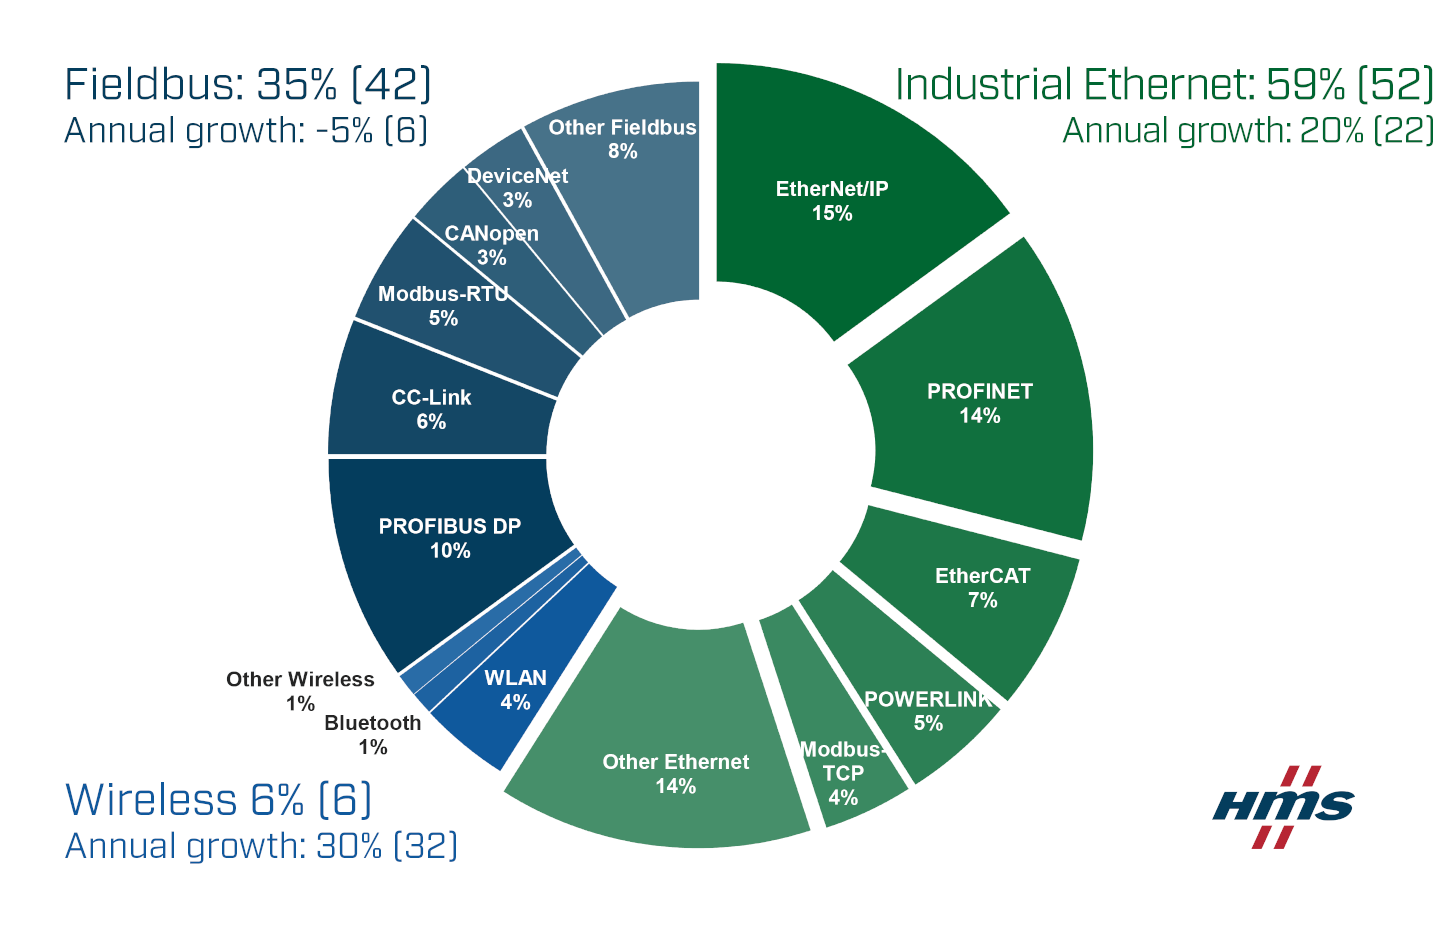
\includegraphics[width=\textwidth]{LPWAN/Figs/networkshares2019.png}
    \end{figure} 
    
    Nasazení bezdrátových technologií ovšem nemá za cíl zcela nahradit komunikaci drátovou. Pro průmyslovou automatizaci, řídící aplikace a real-timové procesy s vysokými nároky na spolehlivost jako je řízení výrobních linek, budou i nadále upřednostňovány spolehlivé a roky odzkoušené protokoly jako PROFINET či ProfiBus.\\
    Pro monitorovací aplikace v~rámci CBM, jež vyžadují připojení velkého množství senzorů, jsou ale tyto technologie příliš těžkopádné a drahé. Hlavní problém také představuje fakt, že v~mnoha případech není možné zasahovat do již fungují komunikační infrastruktury, odstavovat výrobu, a proto převládá snaha novými senzory pouze doplnit stávající řešení \cite{website:3}.\\
    Jsou to tedy především jednoduchost instalace, dosah a spotřeba, proč se v~posledních letech mohutně využívají ve výrobních prostředích bezdrátové sítě. 

\section{LPWAN mezi bezdrátovými IIoT sítěmi}
\label{section:lpwan}
    LPWAN (Low Power Wide Area Network) je rodina bezdrátových sítí určená pro vysoký dosah, nízký datový tok a nízkou energetickou spotřebu, a zejména tak vhodná pro bateriová zařízení. LPWAN technologie také využívají k~připojení zařízení menší šířku frekvenčního pásma, než je obvyklé u~běžně využívaných zařízení u mobilních sítí \cite{website:3}.\\
    Hlavními a prvotními zástupci LPWAN sítí jsou LoRa a SigFox, které jsou provozovány v~bezlicenčních ISM pásmech na kmitočtech 863-870 MHz v~Evropě a 902-928 MHz v~USA \cite{website:5}.\\
    Dále síť NB-IoT fungující v~licencovaných pásmech vlastněných mobilními operátory, kterou proto lze provozovat na již existující mobilní komunikační infrastruktuře pouhou softwarovou úpravou, kdy se vysílacím stanicím vyhradí speciální část pásma. Na rozdíl od sítí Sigfox a LoRa tedy není nutné instalovat žádné dodatečné vysílače \cite{website:4}.
    
    
    LPWAN sítě řeší mnoho problémů, se kterými se potýkají sítě krátkého dosahu (WiFi, Bluetooth\ldots) a celulární mobilní sítě (GSM, GPRS, LTE\ldots). Umožňují bezdrátové připojení senzorů a monitorování i na rozlehlých plochách s velkými vzdálenostmi (stavební plochy, větrné elektrárny) nebo obtížně dostupných místech (malé vodní elektrárny \cite{website:2}, kryty, tunely), kde nasazení monitorovacích systémů nebylo dříve možné nebo bylo velmi finančně nákladné.
    
    
    Ve srovnání s WiFi a Bluetooth je jejich hlavní výhodou především zmíněný vyšší dosah, propustnost ve vnitřních prostorách (tzv. building penetration). U~sítě LoRa pak také díky komunikaci v~rozprostřeném spektru odolnost vůči úzkopásmovému elektromagnetickému rušení, které představuje problém nejen díky přeplnění WiFi kanálů, ale také kvůli průmyslovým strojům jako jsou vysokozdvižné vozíky, jež by často ani neprošly kontrolami EMC.\\
    Hlavním benefitem na rozdíl od mobilních sítí je zejména výdrž baterie. Často se také může stát, že rádiový signál je částečně odstíněn krytem výrobní haly, což lze u LPWAN sítí snadněji vyřešit nasazením brány do vnitřku budovy než u mobilních sítí.

    
\section{Komunikační řetězec LPWAN sítě}
    \begin{figure} [!ht]
        \centering
        \caption{Komunikační řetězec LPWAN sítí. Převzato z \cite{website:4}.}
        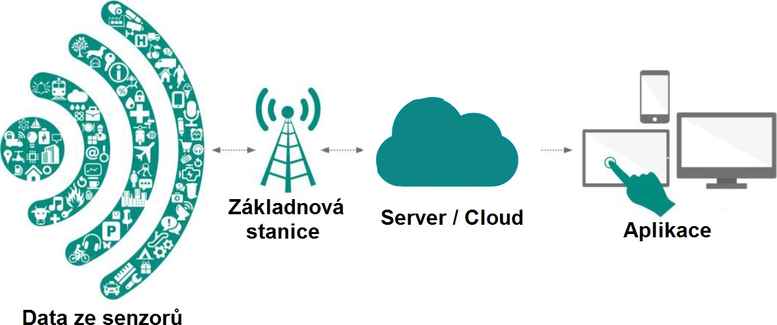
\includegraphics[width=\textwidth]{LPWAN/Figs/communication_chain.png}
    \end{figure} 
    LPWAN síť je tvořená z koncových uzlů využívajících určitý komunikační protokol a odesílajících data do základových stanic (bran), jež data dále přeposílají na vzdálený server, na který jsou napojené aplikace koncových zákazníků.\\
    Uvedené příklady LPWAN sítí (LoRa, Sigfox, NB-IoT) využívají hvězdicovitou topologii \cite{website:4}, kde jednotlivé uzly komunikují vždy pouze s branami, což usnadňuje řízení chodu sítě (není třeba používat složité směrovací protokoly) a usnadňuje její rozšiřování. Středem sítě je poté řídící server, který zajišťuje směrování paketů danému adresátovi.
    
\section{$\text{LoRa}^{\text{TM}}$}
    LoRa, představující zkratku pro slova Long Range, je jeden z hlavních zástupců LPWAN sítí a současně označení pro fyzickou (PHY) vrstvu této proprietární technologie vlastněné francouzskou firmou Semtech. Linková (MAC) vrstva poté nese označení LoRaWAN .\\
    Fyzická vrstva sítě LoRa využívá modulaci s rozprostřeným spektrem, konkrétně variantu modulace CSS (Chirp Spread Spectrum), kdy je přenášená informace modulována na nosný signál, který je lineárně rozmítán od vrchní hranice pásma (bandwidth) po jeho spodní hranici. Strmost tohoto rozmítání určuje parametr označovaný jako Sperading Factor (česky činitel rozprostření, dále pouze jako SF), který tak ovlivňuje rychlost komunikace \cite{manual:1}.\\
    
    \begin{figure} [!ht]
        \centering
        \caption{LoRa modulace – porovnání strmosti rozmítání SF 7-12. Převzato z \cite{picture_website:1}.}
        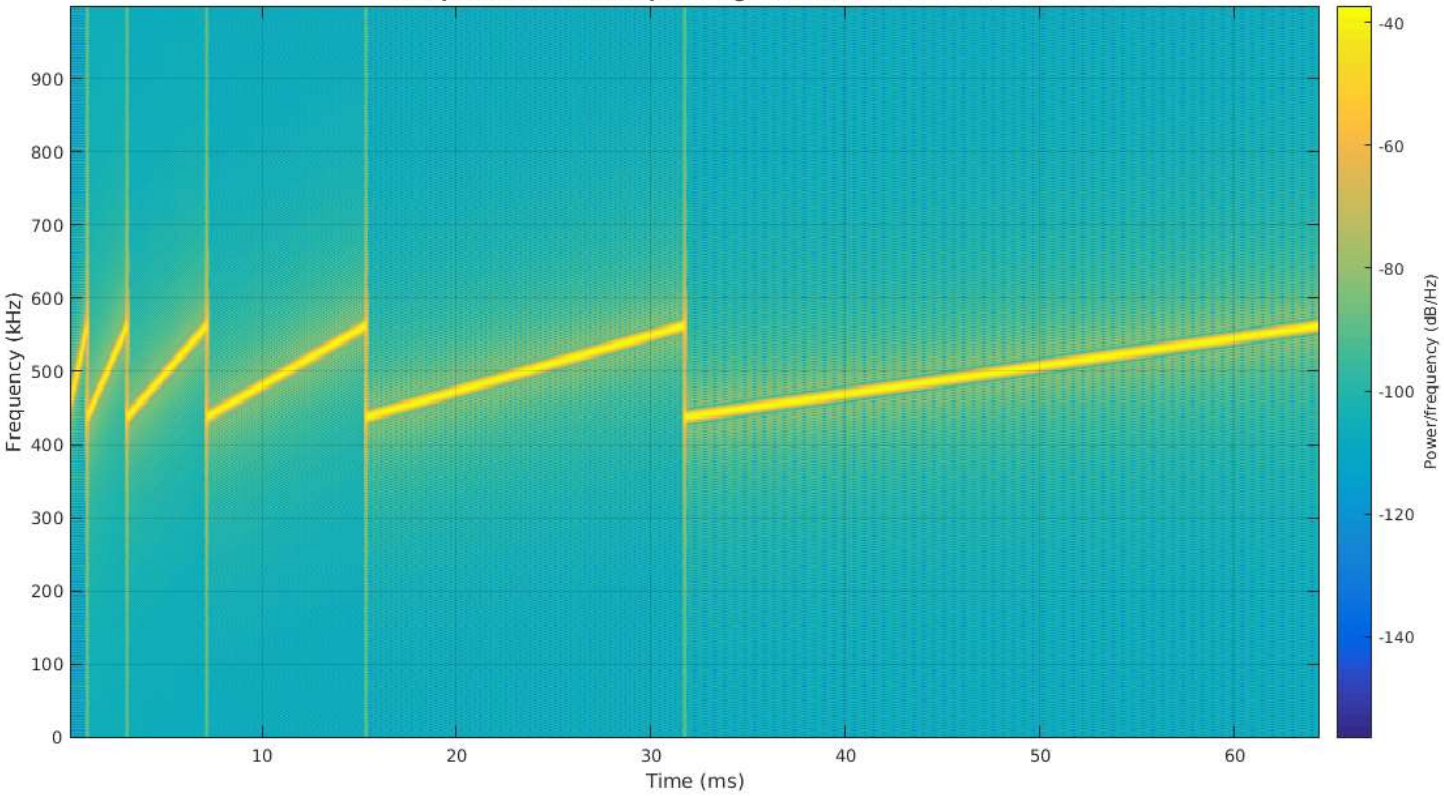
\includegraphics[width=0.9\textwidth]{LPWAN/Figs/lora_sf.png}
    \end{figure} 
    
    Komunikace v~rozprostřeném spektru byla původně vytvořena kvůli vojenským účelům pro minimalizaci možnosti odposlechu, ale dnes se tato technika využívá zejména díky odolnosti vůči úzkopásmovému rušení. Další výhodou jsou samoopravné kódy FEC (Forward Error Correction), větší dosah (ve volném prostranství kolem 10 km) s možností přijímat vysílaný signál až 20 dB pod úrovní šumu, odolnost vůči Doplerovu jevu a potřeba menšího vysílacího výkonu redukujícího spotřebu energie \cite{manual:1}.
    
    \begin{figure} [!ht]
        \centering
        \caption{Komunikace pod úrovní hladiny šumu. Převzato z \cite{picture_website:2}.}
        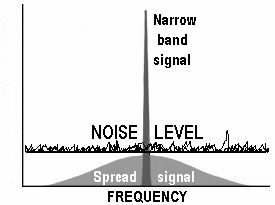
\includegraphics[width=0.6\textwidth]{LPWAN/Figs/lora_noise.jpg}
    \end{figure} 
    

\section{LoRa jako použítá LPWAN síť}
\label{section:single_channel_gw}
    I přes značné výhody NB-IoT v~podobě přenosové rychlosti a pokrytí byla nakonec pro účely této práce  jako komunikační médium zvolena síť LoRa a to především díky ceně rádiových čipů, které jsou kvůli využití bezlicenčních pásem řádově menší.
    
    Mezi cíle práce patří také vytvořit soběstačný systém komunikující oběma směry, nezávislý na pokrytí oficiálních LoRa bran, a proto bylo nutné vytvořit i vlastní bránu.\\
    Kvůli cenovým důvodům navržená brána využívá LoRa čip určený pro koncová zařízení, jehož nevýhoda oproti čipům pro oficiální brány spočívá v~možnosti komunikovat v~danou chvíli pouze na jednom kanálu, a jedná se tak pouze o~tzv. jednokanálovou bránu – anglicky Single channel gateway (více v~kapitole \ref{section:semtech_chips}). Využívaný komunikační kanál a spreading factor tedy musí být u uzlu a jednokanálové brány pro úspěšnou komunikaci předem určen, a nemá smysl proto implementovat LoRaWAN protokol.
    
      \begin{figure} [!ht]
        \centering
        \caption{Oficiální LoRa brána od firmy Multitech využívající čipy SX13xx. Převzato z \cite{website:10}.}
        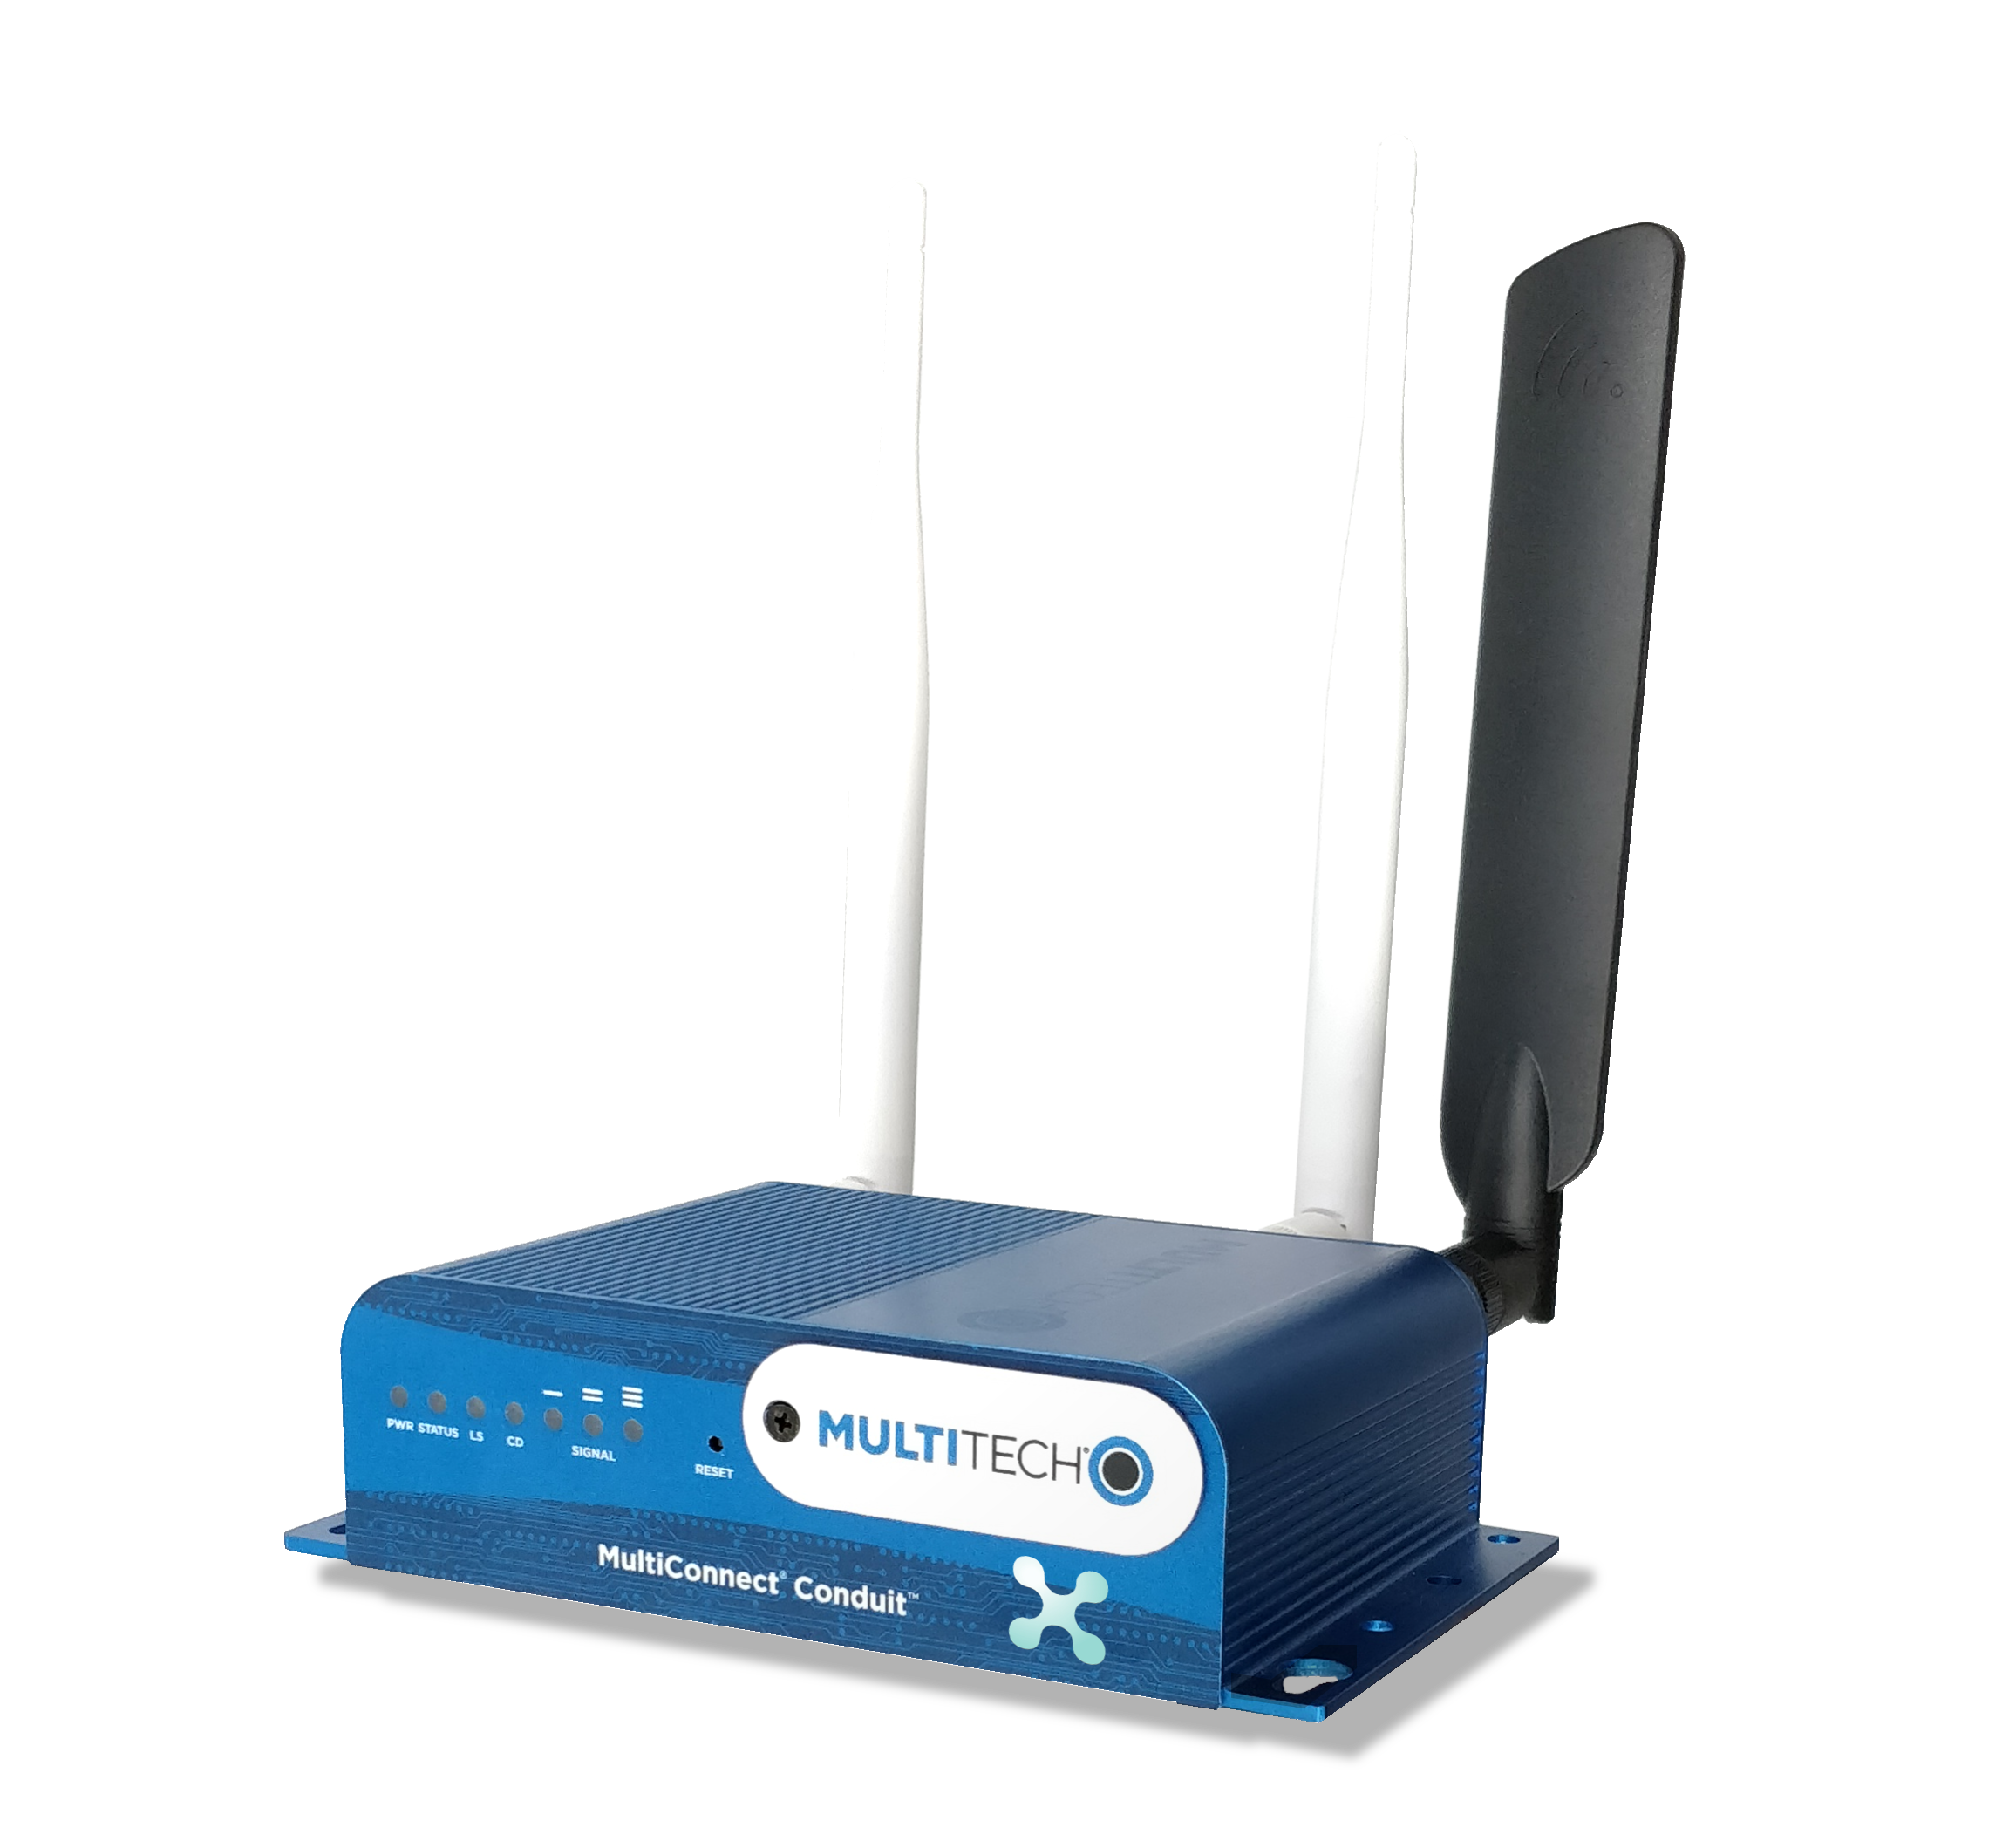
\includegraphics[width=0.8\textwidth]{LPWAN/Figs/lorawan_gw.png}
    \end{figure} 
    
%CHECK ~
%CHECK red
%CHECK ...



% ZDROJE
% https://www.designworldonline.com/industrial-ethernet-takes-the-lead-over-fieldbuses-says-study/

% https://www.automation.com/automation-news/article/lpwan-as-the-new-sensor-communication-infrastructure-for-iiot

% https://www.thethingsnetwork.org/docs/lorawan/frequency-plans.html

% https://elektro.tzb-info.cz/informacni-a-telekomunikacni-technologie/16519-site-pro-internet-veci-v-ceske-republice

% [5]
% https://www.link-labs.com/blog/iot-topology

% [6]
% Rashmi Sharan Sinha, Yiqiao Wei, and Seung-Hoon Hwang. A survey on
% LPWAN technology: LoRa and NB-IoT. ICT Express, 3(1):14–21, 3 2017

% [7] https://www.semtech.com/uploads/documents/an1200.22.pdf
% LPWAN obrazek
% https://medium.com/coinmonks/lpwan-lora-lorawan-and-the-internet-of-things-aed7d5975d5d

% LoRa chirp
% https://fenix.tecnico.ulisboa.pt/downloadFile/1689468335603030/LoRaWAN\%20Introduction.pdf


% https://www.semtech.com/

% Noise 
% https://www.instructables.com/id/Introducing-LoRa-/